% !TEX root = task4.tex
% -----------------------------------------------------------------
% Filename  :	task4_stateMachine_writeAllocatePolicy.tex
% Author    :	Carsten Hoppe
% Date		:	28. Januar 2017
% Reference	:	http://www.texample.net/tikz/examples/state-machine/
%				https://martin-thoma.com/how-to-draw-a-finite-state-machine/
% -----------------------------------------------------------------
%\tikzstyle{every state}=[fill=mycolor,text=white,minimum width=2cm]

In figure \ref{tik:FSM} the state diagram of the cache controller is illustrated. The state diagram represents a Mealy automaton. The state space of the state machine is given in table \ref{tab:tableFSMStates}.
Besides the state machine inputs are listed in table \ref{tab:tableFSMInputs} and the state machine outputs are shown in table \ref{tab:tableFSMOutputs}. A sketch of the state diagram is printed in figure \ref{fig:sketchMealyAutomata}.



\begin{figure}
	\centering
	\caption{State diagram of the cache controller.}
    \label{tik:FSM}
\begin{tikzpicture}[->,>=stealth',shorten >=1pt,auto,
                    semithick,/tikz/initial text=Reset]
                    
    
	% ------------------------------------------------------------------------------
    % Definition of tikz styles.       
	% ------------------------------------------------------------------------------
	\tikzstyle{vertex}=[state,fill=mycolor,text=white,minimum width=1cm]
	\tikzstyle{edge}  =[draw,thick,->, midway, above, sloped]
	
	% ------------------------------------------------------------------------------
	% Definition of nodes.
	% ------------------------------------------------------------------------------
	[align=center,xscale=1,node distance=2cm and 4cm]
	\node[initial,vertex]	(A)                    		{\tiny $IDLE$};
  	\node[vertex]         	(B) [below left=6cm of A] 	{\tiny $CW$};
  	\node[vertex]         	(C) [below=6cm of B] 		{\tiny $CMW$};
  	\node[vertex]         	(D) [below left=4cm of C] 	{\tiny $WBW$};
  	\node[vertex]         	(E) [below right=5cm of D] 	{\tiny $WCW$};
  	\node[vertex]		    (F) [below right=6cm of A] 	{\tiny $CR$};
  	\node[vertex]		    (G) [below =6cm of F] 		{\tiny $CMR$};
  	\node[vertex]		    (H) [below right=4cm of G] 	{\tiny $WBR$};
  	\node[vertex]		    (I) [below left=5cm of H] 	{\tiny $WCR$};

	% ------------------------------------------------------------------------------
	% Definition of paths.
	% ------------------------------------------------------------------------------
	\path (A) [edge] 			  	edge [bend right] node 	{wrCPU='1'/-} 								(B)
		  (B) [edge] 				edge node 				{cacheMiss='1'/stallCPU='1'} 				(C)
		  (B) [edge] 				edge [bend right] node 	{cacheHit='1'/dataCPU2Cache, setDirty='1'} 	(A)
		  (C) [edge] 				edge node 				{isDirty='1'/wrMEM='1'} 					(D)
		  (C) [edge] 				edge node 				{isDirty='0'/rdMEM='1'} 					(E)
		  (D) [edge] 				edge node 				{readyMEM='1'/rdMEM='1'} 					(E)
		  (E) [edge] 				edge node 				{readyMEM='1'/dataCPU2Cache, setDirty='1'} 	(A);
	\path (D) [edge,loop below]		edge node				{readyMEM='0'/-}							(D);
	\path (E) [edge,loop below]		edge node 				{readyMEM='0'/-} 							(E);
		  
	\path (A) [edge] 				edge [bend left] node 	{rdCPU='1'/-} 								(F)
		  (F) [edge] 				edge node 				{cacheMiss='1'/stallCPU='1'} 				(G)
		  (F) [edge] 				edge [bend left] node 	{cacheHit='1'/dataCPU} 						(A)
		  (G) [edge] 				edge node 				{isDirty='1'/wrMEM='1'} 					(H)
		  (G) [edge] 				edge node 				{isDirty='0'/rdMEM='1'} 					(I)
		  (H) [edge] 				edge node 				{readyMEM='1'/rdMEM='1'} 					(I)
		  (I) [edge] 				edge node 				{readyMEM='1'/dataCPU} 						(A);
	\path (H) [edge,loop below] 	edge node 				{readyMEM='0'/-} 							(H);
	\path (I) [edge,loop below]		edge node 				{readyMEM='0'/-}							(I);

		
\end{tikzpicture}
\end{figure}


\begin{table}
\caption{Overview - FSM States}
\label{tab:tableFSMStates}
\begin{tabular}{llll}
\hline %\toprule
Abbreviation & Name & CPU Request Mode & Description \\
\hline %\midrule
IDLE 	& -					& - 			& - \\
CW		& COMPARE WRITE		& Write Request & - \\
CMW		& CACHE MISS WRITE	& Write Request & - \\
WBW		& WRITE BACK WRITE	& Write Request & - \\
WCW		& WRITE CACHE WRITE	& Write Request & - \\
CR		& COMPARE READ		& Read Request 	& - \\
CMR		& CACHE MISS READ	& Read Request 	& - \\
WBR		& WRITE BACK READ	& Read Request 	& - \\
WCR		& WRITE CACHE READ	& Read Request 	& - \\
\hline %\bottomrule
\end{tabular} 
\end{table}

\begin{table}
	\caption{Overview - FSM Inputs}
	\label{tab:tableFSMInputs}
	\begin{tabular}{lll}
	\hline % \topline
	Abbreviation & Name & Description \\
	\hline % \midrule
	rdCPU 		& CPU Read Request			& - \\
	wrCPU 		& CPU Write Request 		& - \\
	cacheMiss 	& Cache Miss 				& - \\
	cacheHit	& Cache Hit					& - \\
	readyMEM 	& Write-Back is resolved 	& - \\
	isDirty		& Cache Block is dirty		& - \\
	\hline % \bottomrule
	\end{tabular}
\end{table}
	
\begin{table}
	\caption{Overview - FSM Outputs}
	\label{tab:tableFSMOutputs}
	\begin{tabular}{lll}
	\hline % \topline
	Abbreviation & Name & Description \\
	\hline % \midrule
	stallCPU		& Stall Processor				& - \\
	setDirty		& Set Dirty Bit (Modified) Bit 	& - \\
	wrMEM			& Write To Memory				& Write Replaced Block To Memory \\
	dataCPU			& Read Data Into CPU			& - \\
	rdMEM			& Read Cache Block Into Cache From Memory & - \\
	dataCPU2Cache	& Write Data Into Cache			& - \\
	\hline % \bottolrule
	\end{tabular}
\end{table}


\begin{figure}
	\centering
	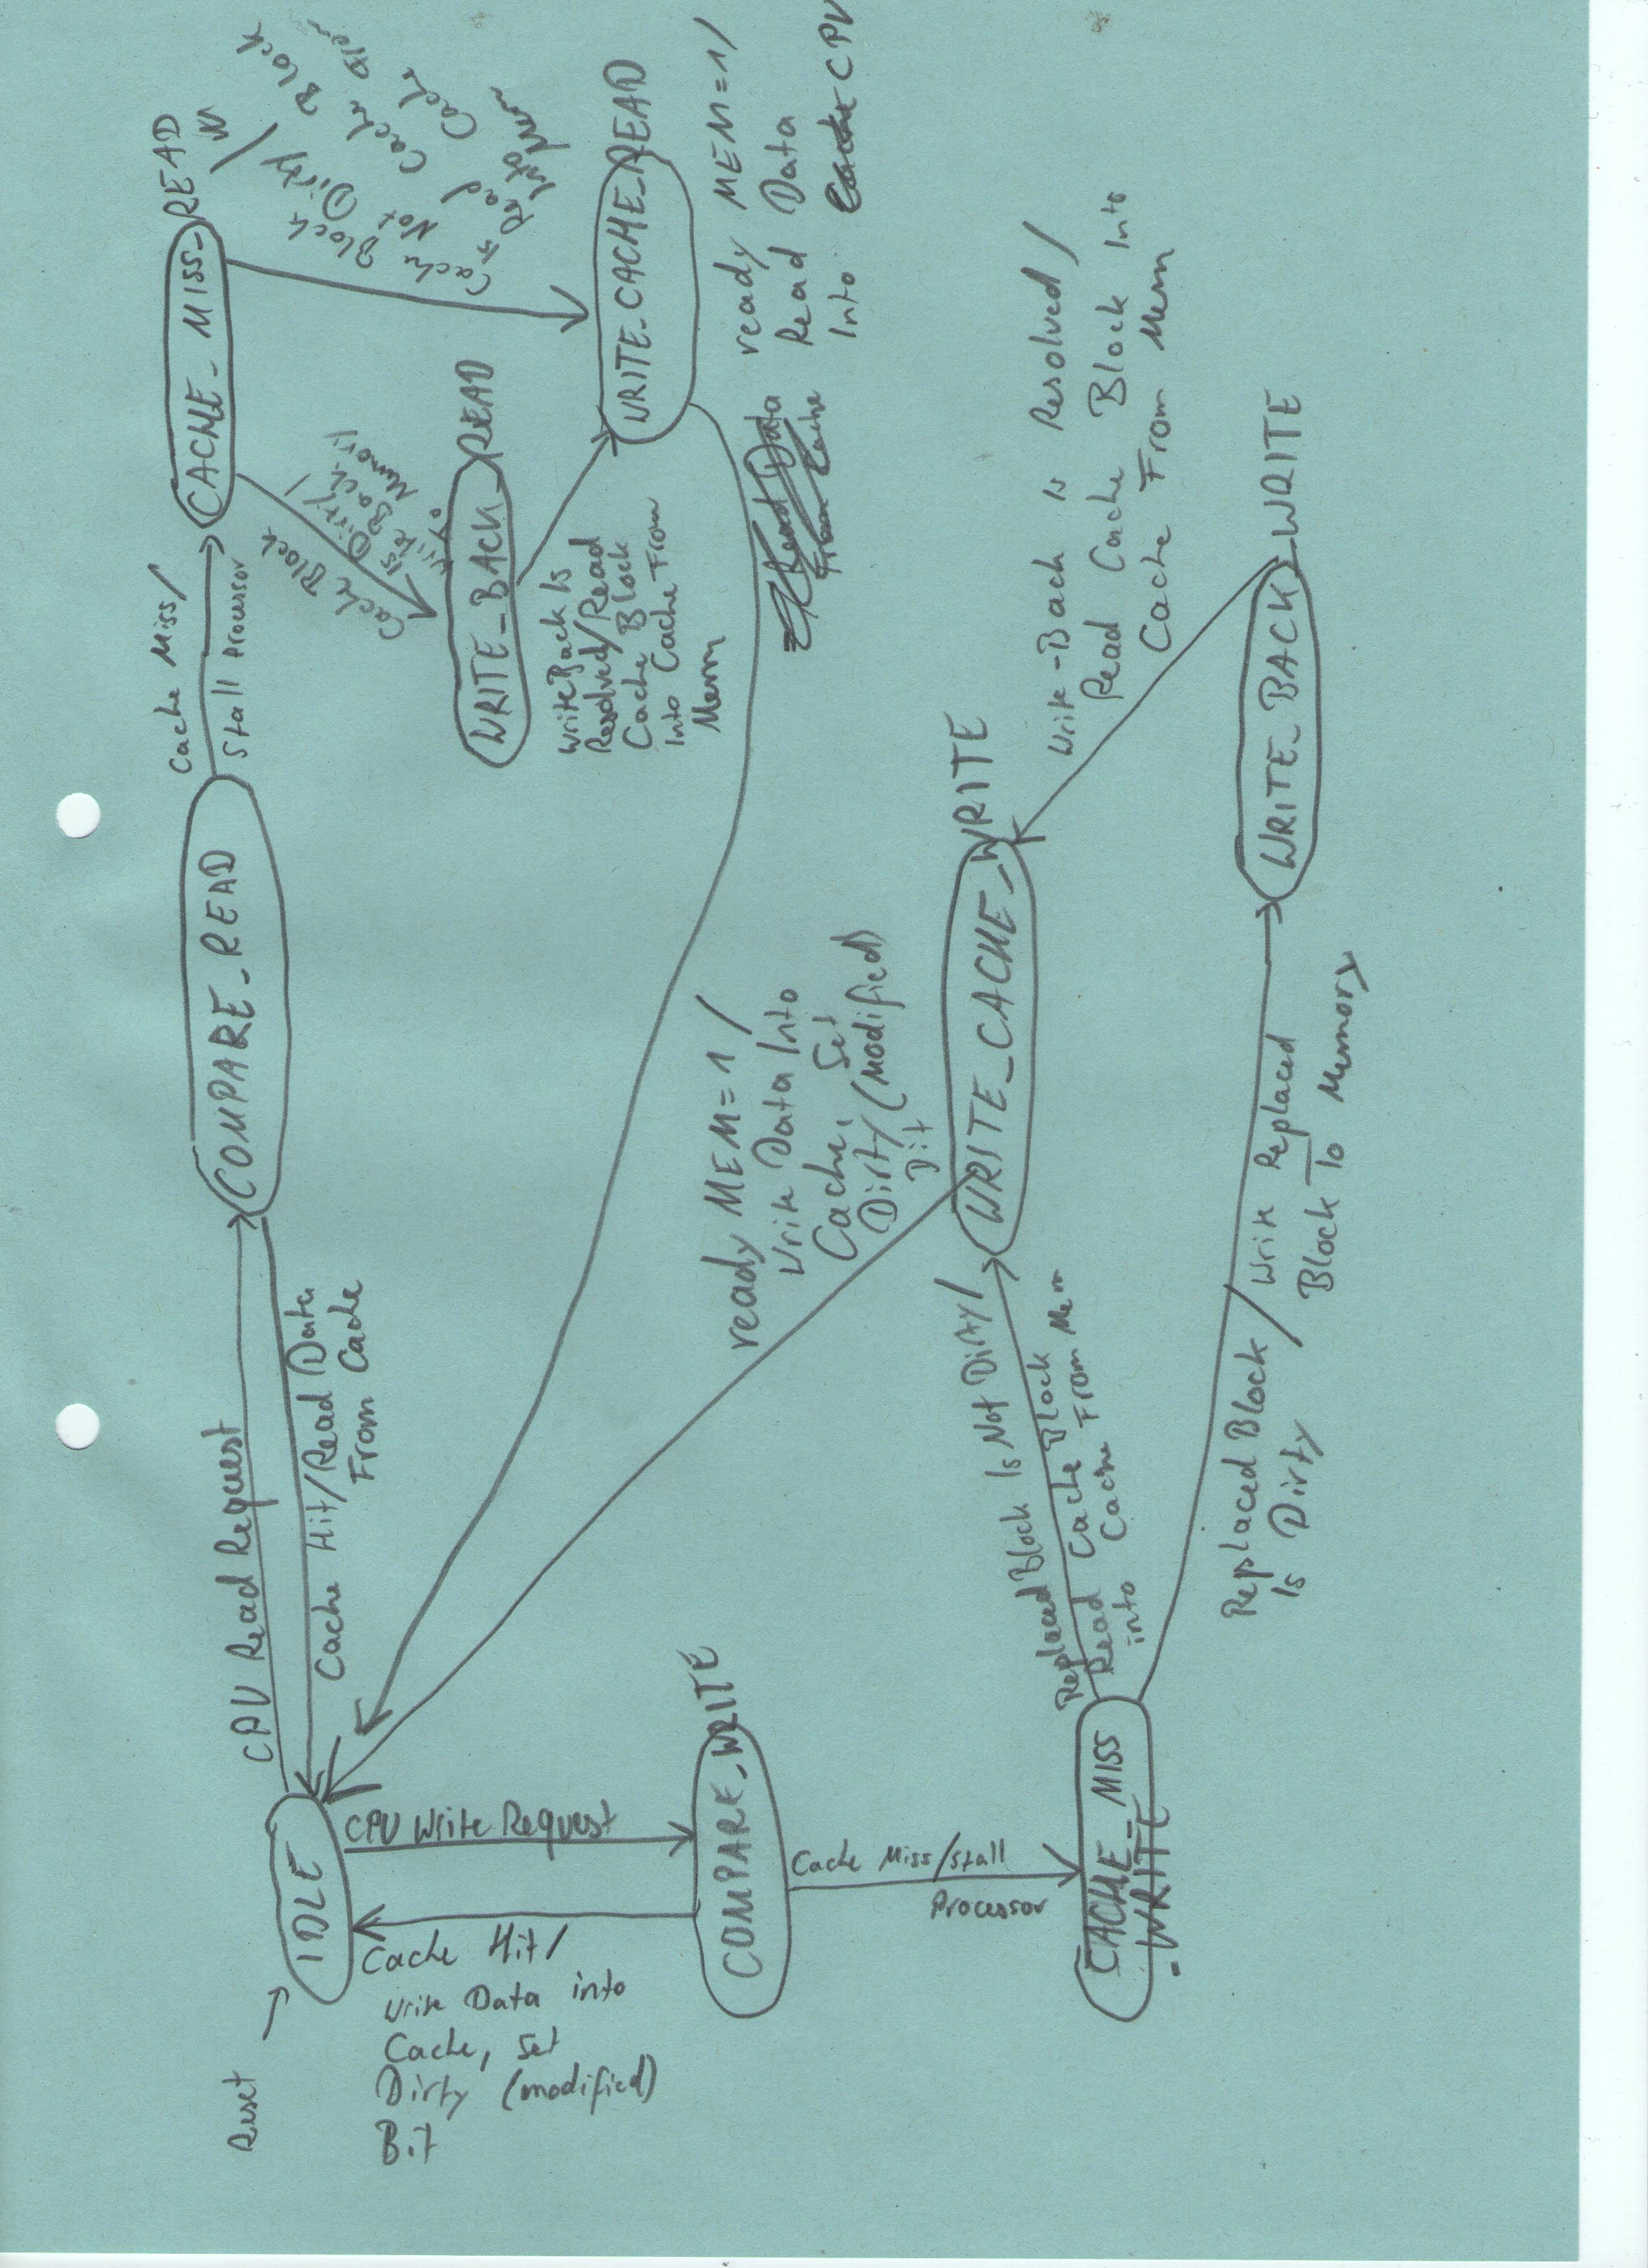
\includegraphics[scale=.8]{pictures/sketch_mealyAutomata}
	\caption{Sketch of Mealy Automata - Cache Controller}
	\label{fig:sketchMealyAutomata}
\end{figure}
